\documentclass[a4paper]{article}
%\usepackage{vntex}
%\usepackage[english,vietnam]{babel}
%\usepackage[utf8]{inputenc}

%\usepackage[utf8]{inputenc}
%\usepackage[francais]{babel}
\usepackage{a4wide,amssymb,epsfig,latexsym,multicol,array,hhline,fancyhdr}

\usepackage{verbatim}
\usepackage{amsmath}
\usepackage{lastpage}
\usepackage[lined,boxed,commentsnumbered]{algorithm2e}
\usepackage{enumerate}
\usepackage{color}
\usepackage{graphicx}							% Standard graphics package
\usepackage{array}
\usepackage{tabularx, caption}
\usepackage{multirow}
\usepackage{multicol}
\usepackage{rotating}
\usepackage{graphics}
\usepackage{geometry}
\usepackage{setspace}
\usepackage{epsfig}
\usepackage{tikz}
\usepackage{ltablex}
\usepackage{enumitem}
\usetikzlibrary{arrows,snakes,backgrounds}
\usepackage{hyperref}
\usepackage{color, colortbl}
\hypersetup{urlcolor=blue,linkcolor=black,citecolor=black,colorlinks=true} 
%\usepackage{pstcol} 								% PSTricks with the standard color package


%\usepackage{fancyhdr}
\setlength{\headheight}{40pt}
\pagestyle{fancy}
\fancyhead{} % clear all header fields
\fancyhead[L]{
 \begin{tabular}{rl}
    \begin{picture}(25,15)(0,0)
    \put(0,-8){
\includegraphics[width=8mm, height=8mm]{hcmut.png}}
    %\put(0,-8){\epsfig{width=10mm,figure=hcmut.eps}}
   \end{picture}&
	%
\includegraphics[width=8mm, height=8mm]{hcmut.png} & %
	\begin{tabular}{l}
		\textbf{\bf \ttfamily Ho Chi Minh University of Technology}\\
		\textbf{\bf \ttfamily Faculty of Computer Science and Engineering}
	\end{tabular} 	
 \end{tabular}
}
\fancyhead[R]{
	\begin{tabular}{l}
		\tiny \bf \\
		\tiny \bf 
	\end{tabular}  }
\fancyfoot{} % clear all footer fields
\fancyfoot[L]{\scriptsize \ttfamily Operating System Lab}
\fancyfoot[R]{\scriptsize \ttfamily Page {\thepage}/\pageref{LastPage}}
\renewcommand{\headrulewidth}{0.3pt}
\renewcommand{\footrulewidth}{0.3pt}


%%%
\setcounter{secnumdepth}{4}
\setcounter{tocdepth}{3}
\makeatletter
\newcounter {subsubsubsection}[subsubsection]
\renewcommand\thesubsubsubsection{\thesubsubsection .\@alph\c@subsubsubsection}
\newcommand\subsubsubsection{\@startsection{subsubsubsection}{4}{\z@}%
                                     {-3.25ex\@plus -1ex \@minus -.2ex}%
                                     {1.5ex \@plus .2ex}%
                                     {\normalfont\normalsize\bfseries}}
\newcommand*\l@subsubsubsection{\@dottedtocline{3}{10.0em}{4.1em}}
\newcommand*{\subsubsubsectionmark}[1]{}
\makeatother

\definecolor{Gray}{gray}{0.9}

\begin{document}

\begin{titlepage}
\begin{center}
HO CHI MINH UNIVERSITY OF TECHNOLOGY \\
FACULTY OF COMPUTER SCIENCE AND ENGINEERING 
\end{center}

\vspace{1cm}

\begin{figure}[h!]
\begin{center}

\includegraphics[width=3cm]{hcmut.png}
\end{center}
\end{figure}

\vspace{1cm}


\begin{center}
\begin{tabular}{c}
\multicolumn{1}{c}{\textbf{{\Large OPERATING SYSTEM LAB (CO2018)}}}\\
~~\\
\hline
\\
\textbf{{\Huge LAB 7 : SCHEDULING}}\\
%\textbf{{\Large (Submission 1)}}\\
\\
\hline
\end{tabular}
\end{center}

\vspace{3cm}

\begin{table}[h]
\begin{tabular}{rrl}
\hspace{5 cm} & Teacher: & Tran Truong Tuan Phat\\
& Student: & Thai Phuc Hiep - 1812227 \\
\end{tabular}
\end{table}

\vspace{4.7cm}

\begin{center}
{\footnotesize HO CHI MINH CITY, June 2020}
\end{center}
\end{titlepage}


%\thispagestyle{empty}

\newpage
\tableofcontents
\newpage

\section{PROBLEM 1 :}
\begin{center}
\begin{tabular}{c|c|c}
Process & Arrival Time & Burst Time \\
\hline
P1 & 0.0 & 8 \\
P2 & 0.4 & 4 \\
P3 & 1.0 & 1 \\
\end{tabular}
\end{center}
\begin{enumerate}[label=\alph*)]
\item FCFS scheduling algorithm \\
\\
Gantt charts : \\
\begin{center}
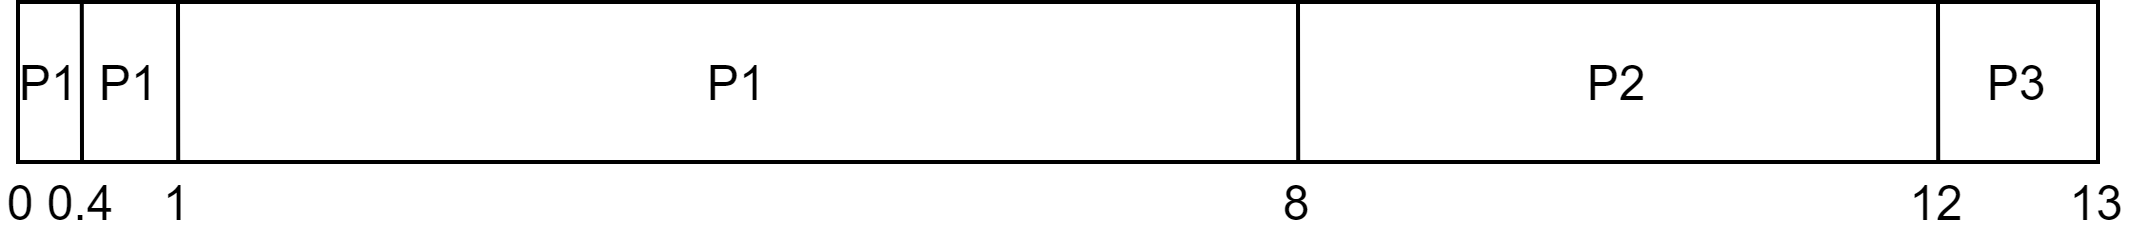
\includegraphics[scale=1]{ex1 fcfs.png}
\end{center}
\begin{center}
\begin{tabular}{|c|c|c|c|c|c|}
\hline
Process & Arrival Time & Completion Time & Turnaround Time \\
\hline
P1 & 0 & 8 & 8 \\
\hline
P2 & 0.4 & 12 & 11.6 \\
\hline
P3 & 1 & 13 & 12 \\
\hline
&&& Average = 10.53 \\ 
\hline
\end{tabular}
\end{center}

\item SJF scheduling algorithm \\
\\
Gantt charts : \\
\begin{center}
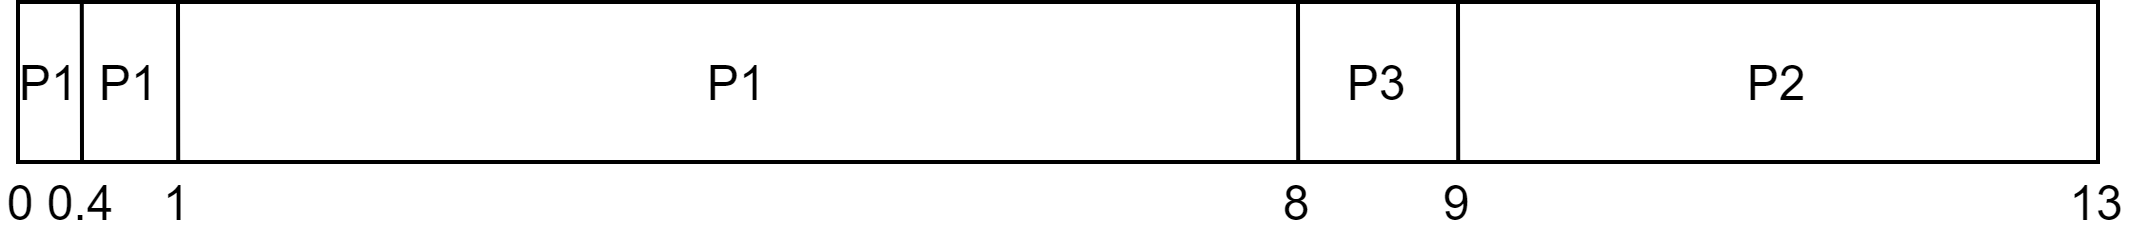
\includegraphics[scale=1]{ex1 sjf.png}
\end{center}
\begin{center}
\begin{tabular}{|c|c|c|c|c|c|}
\hline
Process & Arrival Time & Completion Time & Turnaround Time \\
\hline
P1 & 0 & 8 & 8 \\
\hline
P2 & 0.4 & 13 & 12.6 \\
\hline
P3 & 1 & 9 & 8 \\
\hline
&&& Average = 9.53 \\ 
\hline
\end{tabular}
\end{center}

\item Future-knowledge scheduling algorithm
\\
Gantt charts : \\
\begin{center}
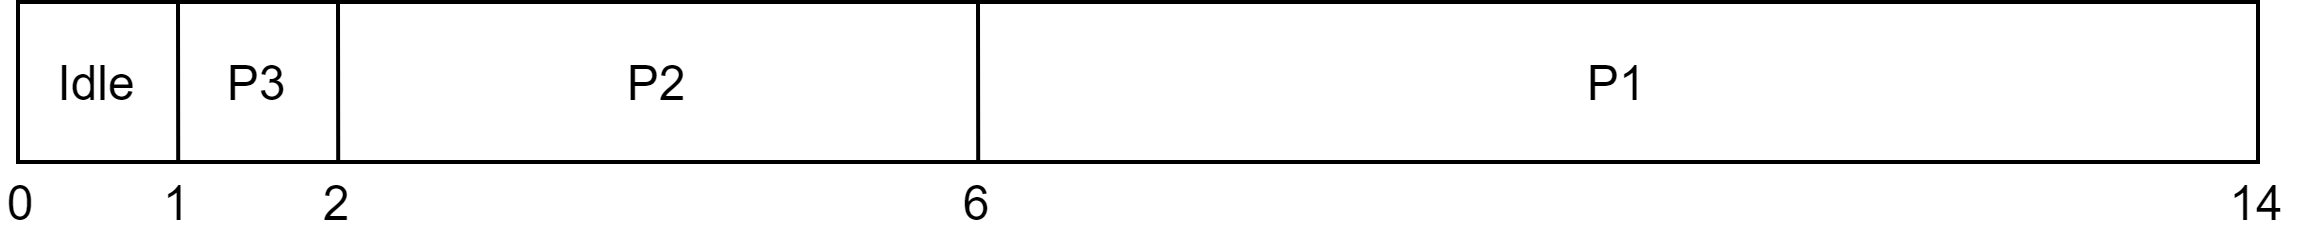
\includegraphics[scale=1]{ex1 future.png}
\end{center}
\begin{center}
\begin{tabular}{|c|c|c|c|c|c|}
\hline
Process & Arrival Time & Completion Time & Turnaround Time \\
\hline
P1 & 0 & 14 & 14 \\
\hline
P2 & 0.4 & 6 & 5.6 \\
\hline
P3 & 1 & 2 & 1 \\
\hline
&&& Average = 6.87 \\ 
\hline
\end{tabular}
\end{center}

\end{enumerate}

\section{PROBLEM 2 :}
\begin{center}
\begin{tabular}{c|c|c}
Process & Burst Time & Priority\\
\hline
P1 & 8 & 4 \\
P2 & 6 & 1 \\
P3 & 1 & 2 \\
P4 & 9 & 2 \\
P5 & 3 & 3 \\
\end{tabular}
\end{center}

\begin{enumerate}[label=\alph*)]
\item FCFS scheduling algorithm \\
\\
Gantt charts :
\begin{center}
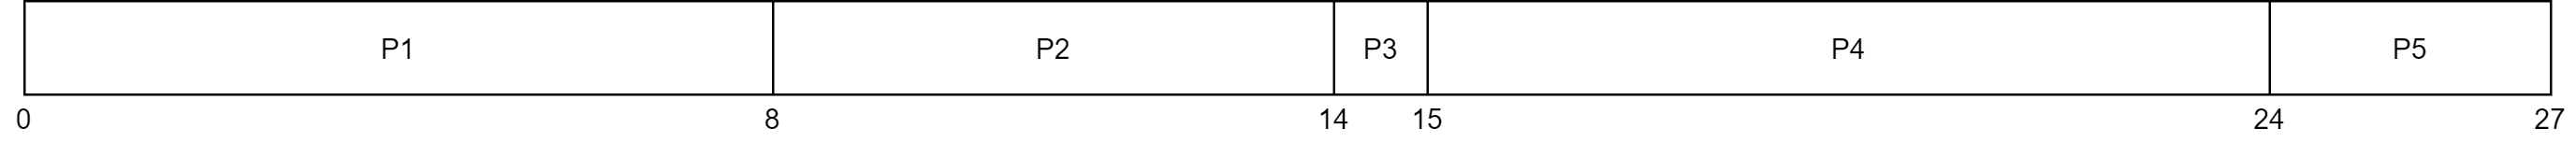
\includegraphics[scale=0.9]{ex2 fcfs.png}
\end{center}
\begin{center}
\begin{tabular}{|c|c|c|c|c|}
\hline
Process & Arrival Time & Completion Time & Turnaround Time & Waiting Time \\
\hline
P1 & 0 & 8 & 8 & 0\\
\hline
P2 & 0 & 14 & 14 & 8\\
\hline
P3 & 0 & 15 & 15 & 14\\
\hline
P4 & 0 & 24 & 24 & 15\\
\hline
P5 & 0 & 27 & 27 & 24\\
\hline
&&& Average = 17.6 & Average = 12.2\\ 
\hline
\end{tabular}
\end{center}

\item SJF scheduling algorithm \\
\\
Gantt charts :
\begin{center}
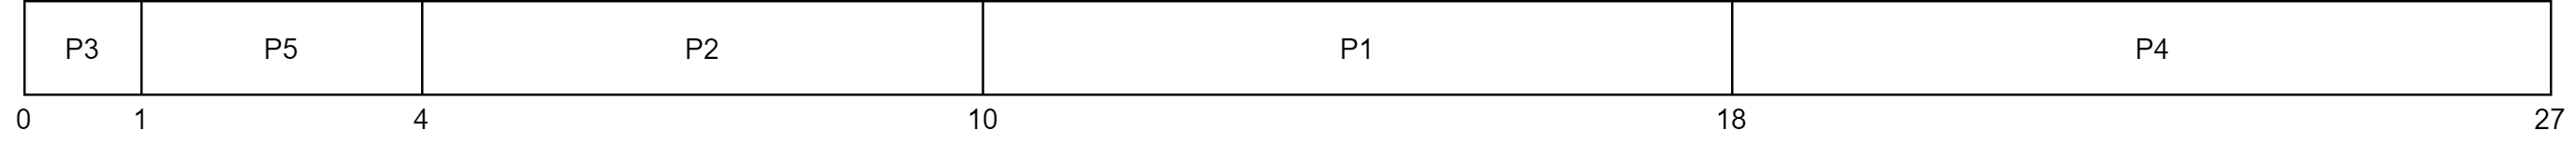
\includegraphics[scale=0.9]{ex2 sjf.png}
\end{center}
\begin{center}
\begin{tabular}{|c|c|c|c|c|}
\hline
Process & Arrival Time & Completion Time & Turnaround Time & Waiting Time \\
\hline
P1 & 0 & 18 & 18 & 10\\
\hline
P2 & 0 & 10 & 10 & 4\\
\hline
P3 & 0 & 1 & 1 & 0\\
\hline
P4 & 0 & 27 & 27 & 18\\
\hline
P5 & 0 & 4 & 4 & 1\\
\hline
&&& Average = 12 & Average = 6.6\\ 
\hline
\end{tabular}
\end{center}

\item Non-preemptive Priority scheduling \\
\\
Gantt charts :
\begin{center}
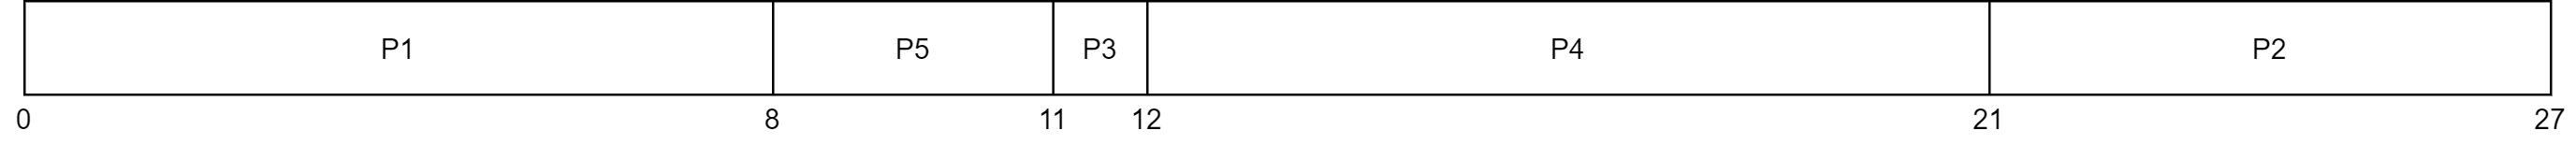
\includegraphics[scale=0.9]{ex2 priority.png}
\end{center}
\begin{center}
\begin{tabular}{|c|c|c|c|c|}
\hline
Process & Arrival Time & Completion Time & Turnaround Time & Waiting Time \\
\hline
P1 & 0 & 8 & 8 & 0\\
\hline
P2 & 0 & 27 & 27 & 21\\
\hline
P3 & 0 & 12 & 12 & 11\\
\hline
P4 & 0 & 21 & 21 & 12\\
\hline
P5 & 0 & 11 & 11 & 8\\
\hline
&&& Average = 15.8 & Average = 10.4\\ 
\hline
\end{tabular}
\end{center}

\item Round-robin scheduling \\
\\
Gantt charts :
\begin{center}
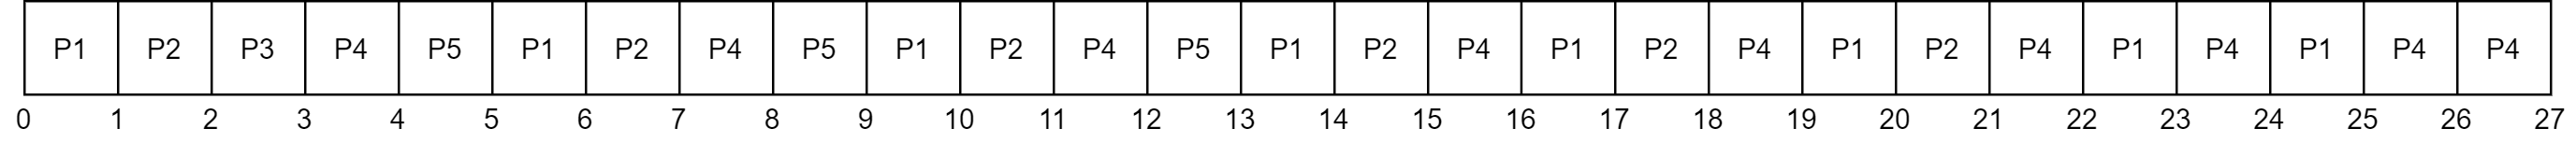
\includegraphics[scale=0.9]{ex2 rr.png}
\end{center}
\begin{center}
\begin{tabular}{|c|c|c|c|c|}
\hline
Process & Arrival Time & Completion Time & Turnaround Time & Waiting Time \\
\hline
P1 & 0 & 25 & 25 & 0\\
\hline
P2 & 0 & 21 & 21 & 0\\
\hline
P3 & 0 & 3 & 3 & 0\\
\hline
P4 & 0 & 27 & 27 & 0\\
\hline
P5 & 0 & 13 & 13 & 0\\
\hline
&&& Average = 17.8 & Average = 0\\ 
\hline
\end{tabular}
\end{center}

\end{enumerate}

\end{document}

